
\documentclass[a4paper,12pt,twoside]{article}
\usepackage[a4paper,top=20mm,bottom=20mm,inner=38mm,outer=19mm]{geometry}
\usepackage{graphicx}
\usepackage{float}
\usepackage{url}
\usepackage{subfigure}
\usepackage[noadjust]{cite}
\usepackage{amssymb}
\usepackage{parskip}
\usepackage{setspace}
\usepackage{listings}
\usepackage{etoolbox}
\patchcmd{\thebibliography}{\section*}{\section}{}{}
\bibliographystyle{apalike} 

\begin{document}
\onehalfspacing

\begin{titlepage}
\clearpage
\vspace*{\fill}
\begin{center}
\begin{minipage}{.6\textwidth}
\centerline{\textbf{\huge Gathering Atmospheric Data}}
\centerline{\textbf{\large Using an Unmanned Air Vehicle}}
\centerline{\textit{Henry Miskin}}
\centerline{\textit{\today}}
\end{minipage}
\end{center}
\vspace{2em}
\centering
\vfill
\textbf{\large Abstract}
\\
This report looked at energy based path planning for atmospheric data collection using unmanned air vehicles in a predetermined area, with particular consideration to the sample quality of data collected. Sampling plans were used in combination with route planning algorithms to produce optimal routes through a sample area. These routes were related to the energy consumed to produce a model that allows energy based path planning. The model for energy based path planning was found to be viable for certain plane configurations.
\vfill
This report is submitted in partial fulfilment of the requirements for the Degree of Bachelor / Master of Engineering, Faculty of Engineering and the Environment, University of Southampton
\clearpage
\end{titlepage}\vfill
\section*{Acknowledgements}
\label{sec:acknowledgements}

I would like to thank my supervisor Andras Sobester for his help and support on this project, firstly by having the confidence in allowing me to explore in a direction that interested me and secondly by offering much needed support at many stages through this process. As a result I have found the work that I have done both interesting and rewarding. I am proud to put my name to this piece of work and know that this would not be the case without the support given.
\vfill\clearpage
\tableofcontents
\vfill
\begin{center}
Word Count: 9924
\end{center}
\vfill
\clearpage
\listoffigures \clearpage

\section*{Abreviations}
ABREVIATIONS-HERE
\section*{Nomeclature}
NOMECLATURE-HERE
\clearpage
\section{Introduction}
\label{sec:introduction}

Unmanned aerial vehicles (UAVs) are used to collect atmospheric data, the flightpath taken by the UAV to collect this data defines where the atmospheric reading of interest is sampled. The locations at which atmospheric data is sampled determines the quality of model that can be produced from the readings. To ensure that the route taken by the UAV is optimal in terms of the quality of data collected, this report utilises optimal sampling plans to define the locations that the UAV should pass through. Then to ensure that the UAV is able to collect as much data as possible, the route through the sample plan is optimised to reduce the energy cost of the route. In this report atmospheric data refers to a meteorological reading to be collected.

\subsection{Aims}
\label{sec:aims}

The aim of this project is to research, design and implement a UAV path planner that minimises energy consumption while optimising spread and depth of data collection.

\subsection{Objectives}
\label{sec:objectives}

The following objectives define the measurable goals of the project required to fully complete the aim. The objectives are listed in the order of completion, where each objective is a prerequisite to the next.

\begin{enumerate}
\setlength{\itemsep}{-12pt}
\item Design a model to calculate the energy costs of flight between two points in space. This model will output the predicted energy required from the work done against drag and the change in gravitational energy.
\item Implement an algorithm that uses the energy model to compare the cost of different routes to result in the least energy consumed.
\item Consider the flight characteristics of the UAV to produce a navigable path which visits the waypoints in order, as defined by the route to produce an accurate flight plan and energy prediction.
\item Fit the results of flight plans in different sample areas to the resulting energy consumed to produce a model that enables optimal path planning based on the area of interest and total UAV energy.

\end{enumerate}

\section{Background Material}
\label{sec:background_material}

\subsection{Problem Outline}
\label{sec:problem_outline}

The troposphere is the lowest atmospheric layer and of significant interest to meteorological researchers as ``almost all weather develops in the troposphere'' \cite{NatGeo}. The section of the troposphere that is closest to the earth is the atmospheric boundary layer, in this layer the atmospheric conditions are affected by the surface of the earth. These effects mean that modelling this section is much more complicated than other layers of the atmosphere, therefore ``the boundary layer is still not represented realistically'' \cite{Teixeira2008}. Developing a greater understanding and thus better modelling of the atmospheric boundary layer will improve the ability to predict weather patterns and pollutant dispersion, to name but two benefits.

To collect atmospheric data a number of approaches have been used historically, ``many years before the use of radio-controlled aircraft, the collection of in-situ measurements was primarily done with balloons, towers, and tethersondes' \cite{Bonin2011}. These options were limited as they were not able to move within the area of interest to build a model. UAVs operate with ``reduced human risk, but also reduced weight and cost, increased endurance, and a vehicle design not limited by human physiology'' \cite{Pepper2012} in comparison to their manned counterparts. This means they provide a cheap and mobile data collection platform.

There are 5 main classes of UAV for different requirements \cite{Sarris2001}; the class of UAV best suited to collecting atmospheric data of a limited area is the close range class. This class of UAV: ``require minimum manpower, training, and logistics, and will be relatively inexpensive'' \cite{FasDod}. These benefits allow a greater number of researchers to have access to mobile data collecting platforms. Most small UAVs are ``not capable of reaching above 5,000ft [1524m]'' \cite{Weibel2005} with their maximum range being less than 10km \cite{Blyenburgh2000}.

\subsection{Literature Review}
\label{sec:literature_review}

To achieve the objectives presented in this project pre-existing material on energy modelling, tour planning, path planning, energy routing and sampling plans has to be considered.

\citen{M.Price2006} consider the design parameters that affect aircraft performance and detail considerations to increase the efficiency. The $L/D$ ratio is identified along with the weight as driving parameters for aircraft range. \citen{Asselin1997} however looks at the top level aerodynamic equations of flight to provide equations capable af defining energy consumption under different flight modes. Together they provide for an overview of flight efficiency and basic equations to estimate this. \citen{Raymer2006} looks further into aerodynamic equations of flight and presents an estimate for the Oswald Factor for standard airframes which is required in a number of the aerodynamic equations.

\citen{Bigg1976,Held1984,DeBerg2010} calculate minimum length tours of more than two points through applying the Travelling Salesperson Problem (TSP). The TSP is concerned with ``finding the shortest path joining all of a finite set of points whose distances from each other are given'' \cite{Held1984}. The TSP problem considered in these papers uses the euclidean distance where the ``euclidean distances satisfy the triangle inequality'' \cite{DeBerg2010}; ``The triangle inequality implies that no reasonable salesman would ever revisit the same city: instead of returning to a city, it is always cheaper to skip the city and to travel directly to the successor city'' \cite{DeBerg2010}. Given the euclidean distances the solutions obtained do not correspond to the shortest path for a either a energy based TSP or a Dubins Travelling Salesman Problem (DTSP)

\citen{Dubins1957,Boissonnat1993} consider the shortest path of a vehicle with a bounded turning radius in two dimensions: given a trajectory and location for the beginning and end points. Both papers found that the minimum path is comprised of maximum rate turns and straight line segments. This initial work on shortest paths is extended by \citen{Chitsaz2007} to take a third dimension into account: for low altitude ranges the shortest path is the Dubins path in the x-y plane and a constant rate altitude climb. High altitude climbs diverged from the Dubins path due to helical climbing component; however this is not relevant as only low altitude climbs are considered in this project.

\citen{McGee2005,Techy2009} apply Dubins shortest path in uniform wind. This is done by considering a ground reference frame and wind reference frame which results in the Dubins minimum path being calculated in the wind reference frame. The maximum rate turns in the air frame of reference ``correspond to trochoidal paths in the inertial (ground) frame'' \cite{Techy2009}. Assuming uniform and time-invariant wind leads to potential inaccuracies which are considered through using 'a turning rate less than the actual maximum turning rate' \cite{McGee2005}. Both papers considered utilise different approaches to obtain a final optimal path, though the resulting optimal paths are both comprised of a combination of trochoidal path sections and straight line sections. These papers present an extension of the Dubins path concept to consider wind but also outline the added complexity of uniform wind without resulting in a vastly different path.

\citen{Savla2005a,Savla2005,LeNy2008} consider the DTSP. The basic approach considered in all papers is in the form of the alternating algorithm which requires calculation of a minimum tour using euclidean distances for an initial ordering. From the initial order the heading at nodes is given by the direction of either the vertex before the node or the vertex after the node. With the order, location and heading defined at each point the Dubins shortest path can be calculated. \citen{Savla2005} goes on to consider stochastic DTSP where the points are normally distributed and puts forth a bead tilling algorithm to improve the performance which is an important consideration for the initial planning aspect of this paper. \citen{LeNy2008} however goes beyond the scope of this paper in considering variable vehicle dynamics.

\citen{Al-Sabban,Chakrabarty2009,Langelaan2007} look into the minimum energy paths through non-uniform wind vectors by considering the total energy of the UAV and attempting to minimise the reduction in energy. \citen{Al-Sabban} uses a markov decision process to plan a route through time varying wind vectors which have a degree of uncertainty. \citen{Chakrabarty2009,Langelaan2007} however use a predetermined knowledge of the wind with the aim to exploit atmospheric energies. The given equations of energy and considerations of optimal routes through complex wind fields applies directly to this paper; however attempting to tap into soaring flight is not feasible given the requirement to fully investigate a particular research area.

\citen{Forrester2008,McKay2000} consider efficient sampling plans for black box experiments to improve the quality of the model produced. Both papers present Latin hypercube sampling to be an improvement on random sampling as they ensure ``that each of those components is represented in a fully stratified manner'' \cite{McKay2000} where those components refer to input dimensions. \citen{Forrester2008} extends this by optimising Latin hypercubes to result in the plan with best space fillingness. The sampling plans provided can easily be utilised in the primary planning component of the UAV tour in this project. \citen{AlexanderI.J.Forrester2009} additionally looks at adding samples to existing surrogates to improve the quality of the model produced. These papers provide the basis for optimal sampling plans for both initial data collection and subsequent flights given an existing model. This outlines the importance of a versatile path planner that can cover an area of interest in addition to any collecting of nodes no matter how sparse.

\section{Background Concepts}
\label{sec:background_concepts}

\subsection{Latin Hypercubes}
\label{sec:latin_hypercubes}

Latin hypercubes are sampling plans that provide the best space fillingness while limiting the total number of sampling points required. This is generally applied to testing of computer simulations where the collection of each point is expensive. In this situation however the travel between the points is the expensive component.

\begin{figure}
	\centering
	
	\subfigure[10 Node Plan]{
		\includegraphics[width=0.44\textwidth]{figures/10_node_plan.png} 
		\label{fig:10_node_plan}
	}
	\subfigure[20 Node Plan]{
		\includegraphics[width=0.44\textwidth]{figures/20_node_plan.png} 
		\label{fig:20_node_plan}
	}
	\subfigure[60 Node Plan]{
		\includegraphics[width=0.44\textwidth]{figures/60_node_plan.png} 
		\label{fig:60_node_plan}
	}
	\subfigure[100 Node Plan]{
		\includegraphics[width=0.44\textwidth]{figures/100_node_plan.png} 
		\label{fig:100_node_plan}
	}
	\caption{Latin Hypercubes with Varying Numbers of Nodes}
	\label{fig:latin_hypercubes_with_varying_numbers_of_nodes}
\end{figure}

Figure \ref{fig:latin_hypercubes_with_varying_numbers_of_nodes} shows Latin hypercubes with varying numbers of nodes. The nodes within the Latin hypercubes are located in such a way that ensures along each vertex the nodes are equally spaced and the spread of the nodes is maximised. The resulting plans are therefore efficient sampling plans that are space filling within the area of interest. The Latin hypercubes shown here are computed within MATLAB using code from the work of \citen{Forrester2008} and imported into python for utilisation within this project. Once a Latin hypercube is computed the result is cached so for any following calls MATLAB is not required to be called.

Given that data collection is rarely within a unit cube and more likely on the scale of thousands of meters in a research area that is far from a cuboid, these sample plans need to be altered for use. To apply these Latin hypercubes to provide sampling plans for any research area they can be stretched in each vertex.

\begin{figure}
	\centering
	
	\subfigure[777 x 925 x 968]{
		\includegraphics[width=0.44\textwidth]{figures/777_x_925_x_968.png} 
		\label{fig:777_x_925_x_968}
	}
	\subfigure[534 x 68 x 506]{
		\includegraphics[width=0.44\textwidth]{figures/534_x_68_x_506.png} 
		\label{fig:534_x_68_x_506}
	}
	\subfigure[71 x 86 x 937]{
		\includegraphics[width=0.44\textwidth]{figures/71_x_86_x_937.png} 
		\label{fig:71_x_86_x_937}
	}
	\subfigure[54 x 543 x 93]{
		\includegraphics[width=0.44\textwidth]{figures/54_x_543_x_93.png} 
		\label{fig:54_x_543_x_93}
	}
	\caption{Stretched 100 Node Latin Hypercubes}
	\label{fig:stretched_100_node_latin_hypercubes}
\end{figure}

Figure \ref{fig:stretched_100_node_latin_hypercubes} shows a number of 100 node Latin hypercubes stretched to varying research areas. It can be seen that the data spread of the Latin hypercubes remains the same along each of the vertexes; however in terms of actual distance between nodes in the sampling plan this causes bunching. This results in data that is equally sampled for each input variable therefore the effect of each variable on the model is equally considered.

\subsection{Exact Travelling Salesman}
\label{sec:exact_travelling_salesman}

To calculate the least cost tour of a number of nodes the TSP presents itself. The TSP is well documented for many route planning problems, both for two dimensions and three dimensions. The standard form of the TSP is to calculate the least cost of visiting every node where the cost is defined as the euclidean distance between nodes. Due to the euclidean properties of the TSP there are many heuristic approaches to computing best guess solutions.

Without the utilisation of heuristic approaches the TSP is a very computationally expensive problem. This is due to the number of routes that are possible given even a small number of nodes. The number of routes increase by a factor of the total number of nodes each time a node is added to the computation. This is due to that new node needing to be considered at every point in every existing route.

\begin{figure}
\centering
\includegraphics[width=0.6\textwidth]{figures/connections_and_shortest_route_through_6_nodes.png} 
\caption{Connections and Shortest Route through 6 Nodes}
\label{fig:connections_and_shortest_route_through_6_nodes}
\end{figure}

Figure \ref{fig:connections_and_shortest_route_through_6_nodes} shows an arrangement of nodes with all possible connections shown in blue and the shortest route in green. The number of connections between 6 nodes route is 15. Given that the number of routes through these connections totals to 720 this shows how the TSP can easily become unmanagable.

The optimal route is a found using python. A matrix of the length of all connections is calculated using the euclidean distance, then the route distances are found from summing up the individual connection distances from the distance matrix. For all permutations of node ordering, the length of the path is computed and the shortest route is selected.

For the route planning in this report it is imperative to devise a TSP solution that provides a best guess method to finding a least cost route. This is because the number of nodes required for a sampling plan to achieve a high quality model will far exceed 10 nodes, resulting in excessive computation time.

\subsection{Dubins Paths}
\label{sec:dubins_paths}

The shortest path between two locations when considering purely a start and end location is the euclidean distance between each node. This is the distance that would be experienced by a vehicle that can travel in any direction regardless of current heading. To work out the path length between two points where the start and end directions are determined is a more complicated problem. This requires the considering of the minimum turning radius for the vehicle in question.

A Dubins path is a minimum distance path between a given start position and direction and a given end position and direction. There are a number of different forms of Dubins paths that can be achieved and the minimum path is the minimum of the Dubins paths that can be computed. These paths are comprised of maximum rate turns and straight line segments.

\begin{itemize}
\setlength{\itemsep}{-12pt}
\item RSR - Right Turn, Straight Travel then Right Turn
\item RSL - Right Turn, Straight Travel then Left Turn
\item LSR - Left Turn, Straight Travel then Right Turn
\item LSL - Left Turn, Straight Travel then Left Turn
\item RLR - Right Turn, Left Turn then Right Turn
\item LRL - Left Turn, Right Turn then Left Turn

\end{itemize}

To calculate the different Dubins paths that are possible geometric relations and vector identities can be utilised. The initial stage is to consider the start and end directions. For both the start and end directions the circles that correspond to maximum rate turns are computed. That is the circle where the initial direction is tangential to the circumference and the circles where the final direction is tangential to their circumference.

These paths are calculated in python using the logic detailed by \citen{Giese2012} to determine the geometric and draw respective paths. The shortest path is then selected by comparing the resulting distances.

For the routes with a straight line segment in the middle, tangent lines are computed. These four sets of lines that are tangential to a start and end circle make up the straight section of the route. The complete path is the combination of an arc that lies in the circumference of the start circle, the straight line section to the end circle and then an arc in the circumference of the end circle. For some cases where the start and end points are close some path types are not achievable.

\begin{figure}
	\centering
	
	\subfigure[Turn Straight Turn]{
		\includegraphics[width=0.44\textwidth]{figures/turn_straight_turn.png} 
		\label{fig:turn_straight_turn}
	}
	\subfigure[Turn Turn Turn]{
		\includegraphics[width=0.44\textwidth]{figures/turn_turn_turn.png} 
		\label{fig:turn_turn_turn}
	}
	\caption{Dubins Paths Comprised of Turns and Straight Line Segments}
	\label{fig:dubins_paths_comprised_of_turns_and_straight_line_segments}
\end{figure}

Figure \ref{fig:turn_straight_turn} shows the possible routes from the point (0, 0) in direction (0, 1) to the point (-4, -2) in direction (1, 0). The arrows symbolise the start and end headings and the different coloured route symbolise the different routes. In this example the routes comprise of maximum rate turns of radius 1 and straight line segment.

To calculate the paths that are comprised of only maximum rate turns the start and end circles are used again. The circles that lie with their circumference tangential to both a start and end circle is used to determine the points of change from one turn direction to the other. The path then follows the circumference of each of the three circles in turn. Paths of only maximum rate turns are only viable when $D<4r$ where $D$ symbolises the distance between the start and end points, as above this distance the radius would need to increase to be navigable using only three circles.

Figure \ref{fig:turn_turn_turn} shows the possible routes from the point (0, 0) in direction (0, 1) to the point (2, -1) in direction (1, 0). The arrows symbolise the start and end headings and the different coloured route symbolise the different routes. In this example the routes only comprise of maximum rate turns of radius 1.

\section{Method}
\label{sec:method}

To achieve the objectives of this project a particular process had to be followed. This ensured that each further level of investigation was based on completion of the one preceding it. The initial goal was to design a simple yet effective energy model that could use actual plane data and return the expected energy consumption for a number of flight manoeuvres. Using this energy model as a basis for comparison the computation time of the TSP needed to be improved. Having obtained a least energy route through a sampling plan then create a path through the route that adheres to the UAV flight characteristics.

In this section and for the remainder of this report, \textbf{route planning} refers to the ordering of nodes within the sample plan and \textbf{path planning} refers to the creating of navigable paths from this ordering of nodes. The route planning aspect requires ranking of comparative energies, however the path planning component requires more detailed energy considerations.

\subsection{Energy Model}
\label{sec:energy_model}

To correctly estimate the energy used in navigating through a particular route, an energy model to define how different flight manoeuvres consume energy was required. For a basis of the energy model the plane was assumed to consume energy in two ways: in doing work against drag and by doing work against gravity. As the plane navigates the manoeuvres on its route the consumption reduces the available energy in the plane's battery. Given a good energy model the length of the route can be determined a priori safe in the knowledge that the plane will not run out of energy before completing its route.

Obtaining accurate values for the variables required for energy modelling is difficult given an off the shelf UAV. Therefore the energy model was harder to calculate for individual planes. To work around this problem the aerodynamic values for the plane were obtained from results to foil simulations from the internet. This enabled a similar airfoil shape to be selected that allows aerodynamic variables to be easily obtained. The website \textit{airfoiltools.com} contains the results to simple simulations on many airfoils and the data can be pulled for virtually any foil shape at varying Reynolds numbers.

\begin{figure}
\centering
\includegraphics[width=1\textwidth]{figures/energy_model_diagram.png} 
\caption{Diagram of Energy Model Logic}
\label{fig:energy_model_diagram}
\end{figure}

Figure \ref{fig:energy_model_diagram} shows the logic behind the approach used to compute an energy model using readily available atmospheric and plane variables. The best Reynolds number was then selected an iterative approach which was used to download airfoil coefficients. The following equations were used to produce the energy model.

\begin{equation}
\label{eq:reynold_number}
Re = \frac{\rho c V}{\mu}
\end{equation}

Equation \ref{eq:reynold_number} was used to calculate the Reynolds number given the flight conditions of the plane. This was required to select the correct data set for obtaining the relevant values for coefficient of lift and the zero lift coefficient of drag.

\begin{figure}
	\centering
	
	\subfigure[Coeficient of Lift $C_L$]{
		\includegraphics[width=0.44\textwidth]{figures/coeficient_of_lift__c_l_.png} 
		\label{fig:coeficient_of_lift_c_l}
	}
	\subfigure[Coefficient of Zero Lift Drag $C_{{D_0}}$]{
		\includegraphics[width=0.44\textwidth]{figures/coefficient_of_zero_lift_drag__c_d_0_.png} 
		\label{fig:coefficient_of_zero_lift_drag_c_d_0}
	}
	\caption{$C_L$ and $C_{D_0}$ Plots of a NACA23015-IL Airfoil}
	\label{fig:c_l_and_c_d_0_plots_of_a_naca23015il_airfoil}
\end{figure}

Figure \ref{fig:c_l_and_c_d_0_plots_of_a_naca23015il_airfoil} shows the coefficient of drag and coefficient of lift for varying angles of attack. This is data obtained directly from \textit{airfoiltools.com} for the NACA23015-IL airfoil operating in conditions with a Reynolds number between 50000 and 1000000.

\begin{equation}
\label{eq:maximum_range_equation}
C_L = \sqrt{C_{D_0}\pi A e}
\end{equation}

Equation \ref{eq:maximum_range_equation} shows the relationship between the coefficient of lift and the zero lift coefficient of drag where the plane's range is a maximum. The data from \textit{airfoiltools.com} was then used to find the values of the coefficients where the equation is satisfied. This calculation was only required if the flight velocity of the plane was not defined.

\begin{equation}
\label{eq:steady_velocity_equation}
V=\sqrt{\frac{2mg}{\rho S C_L}}
\end{equation}

Equation \ref{eq:steady_velocity_equation} depicts the relationship between velocity and the coefficient of lift. This equation was utilised in two ways. When the velocity of the plane is defined this equation defines the coefficient of lift. When however the coefficient of lift is calculated from equation \ref{eq:maximum_range_equation} this equation is used to define the velocity.

\begin{equation}
\label{eq:drag_coeficient}
C_D = C_{D_0} + \frac{C_L^2}{\pi A e}
\end{equation}

Equation \ref{eq:drag_coeficient} was used to amend the coefficient of drag for a 3 dimensional wing. This utilises the Oswald factor and aspect ratio which are parameters used to define the wing loading and shape profile respectively.

\begin{equation}
\label{eq:load_factor_equation}
n=\frac{L}{W}=\sqrt{1+\left(\frac{V^2}{R g}\right)^2}
\end{equation}

Equation \ref{eq:load_factor_equation} shows the relationship between the load factor and the turning radius for the plane. The load factor is the ratio of lift to weight during a turn. This allows the greater energy required in turns to be considered for path planning.

\begin{equation}
\label{eq:level_flight_energy}
E = \frac{1}{2} \rho C_D S V^2 D
\end{equation}

\begin{equation}
\label{eq:turning_flight_energy}
E= n\frac{C_D}{C_L} m g D
\end{equation}

\begin{equation}
\label{eq:climbing_flight_energy}
E = mg H
\end{equation}

Equations \ref{eq:level_flight_energy}, \ref{eq:turning_flight_energy} and \ref{eq:climbing_flight_energy} were used to calculate the level, turning and climbing flight consumption of energy respectively. Climbing flight here only considers the work against gravity. Therefore for any form of climbing flight the energy consumption due to drag must also be taken into account. For example if a plane were to fly $1m$ horizontally and $1m$ vertically then the energy used would be found by summing equation \ref{eq:level_flight_energy} with $D=\sqrt{2}$ and equation \ref{eq:climbing_flight_energy} with $H=1$.

The energy model was then simplified for the route planning. In the route planning the actual energy does not matter but the ranking of energy consumption does. For this reason the accurate equations for energy are reduced to a form where the energy is merely a cost balance between level and climbing flight. This is similar to the $L/D$ ratio.

\begin{equation}
\label{eq:energy_equation}
E =\gamma(\beta D + H)
\end{equation}

\begin{equation}
\label{eq:beta_equation}
\beta = \frac{\rho C_D S V^2}{2mg}
\end{equation}

\begin{equation}
\label{eq:gamma_equation}
\gamma = mg
\end{equation}

Equation \ref{eq:energy_equation} is the overall energy equation used to calculate accurate energy based on distance and height gain. The constants $\beta$ and $\gamma$ are depicted in equations \ref{eq:beta_equation} and \ref{eq:gamma_equation} respectively. The energy model has been manipulated in this way to illustrate that the $\gamma$ component is merely a factor applied to the whole equation. Therefore for the purpose of routing the constant $\alpha$ can be used alone to define the energy equation. This abstraction provides for the constant $\gamma$ to not affect route selection. Therefore it can be applied subsequently to calculating the ordering of nodes.

From this point forward in the report the energy computation will be referred to in two ways: the \textbf{cost} of a route will refer to the component of equation \ref{eq:energy_equation} contained within the brackets and is an adjusted length measured in meters, the \textbf{energy} however refers to the result of the full equation and is measured in joules.

\subsection{Exact Travelling Plane}
\label{sec:exact_travelling_plane}

The exact travelling plane developes on the TSP to include energy considerations for route planning. Firstly the cost of travel between every possible pair of nodes in the sample plan was calculated. Then for every permutation of how these nodes can be ordered the cost of the overall route was calculated and the least cost selected as the optimal route.

\begin{figure}
	\centering
	
	\subfigure[4 Node Route]{
		\includegraphics[width=0.44\textwidth]{figures/4_node_route.png} 
		\label{fig:4_node_route}
	}
	\subfigure[6 Node Route]{
		\includegraphics[width=0.44\textwidth]{figures/6_node_route.png} 
		\label{fig:6_node_route}
	}
	\subfigure[8 Node Route]{
		\includegraphics[width=0.44\textwidth]{figures/8_node_route.png} 
		\label{fig:8_node_route}
	}
	\subfigure[10 Node Route]{
		\includegraphics[width=0.44\textwidth]{figures/10_node_route.png} 
		\label{fig:10_node_route}
	}
	\caption{Exact Travelling Salesman Routes}
	\label{fig:exact_travelling_salesman_routes}
\end{figure}

Figure \ref{fig:exact_travelling_salesman_routes} shows the optimal routes for different numbers of nodes. These optimal routes are found by computing the exact cost of each and every route option. Although this yields the shortest route, this approach was not efficient in terms of the computation time required. To enable calculation of a 10 node route the start point of the route was defined by the lowest node. This reduces the complexity of the path planning problem to that of a 9 node route. 

\begin{table}[width=\textwidth]
\centering

    \begin{tabular}{lllll}
    Number of points	& 4	& 6	& 8	& 10	\\
Number of possible routes	& 6	& 120	& 5040	& 362880	\\
Computation time (ms)	& 0.0	& 1.0	& 43.0	& 3658.0	\\
Best route cost (m)	& 1.16	& 1.11	& 1.11	& 1.14	\\

    \end{tabular}
\caption{Comparison of route calculation}
\label{tbl:comparison_of_route_calculation}
\end{table}

Table \ref{tbl:comparison_of_route_calculation} shows the number of possible routes and the resulting computation time given different numbers of nodes. For a standard travelling salesman problem the number of possible routes is defined by $n!$ however in this case the number of route options is equivalent to $(n-1)!$ where $n$ is the number of nodes in each case. This is due to the start node being defined, thus the complexity is reduced by a single node. The number of routes directly relates to the computation time.

The computation time of the exact TSP far exceeds what would be practical for this project; therefore the performance has to be increased to produce workable routes from the number of nodes required. The heuristic approach used in this report is taken from consideration that the best routes in figure \ref{fig:exact_travelling_salesman_routes} are generally comprised of a single climbing component and single descending component.

\subsection{Progressive Travelling Plane}
\label{sec:progressive_travelling_plane}

From the observation that the optimal routes from figure \ref{fig:exact_travelling_salesman_routes} all comprised of an up component and down component, the logic for a best guess approach was devised with far less computation time required. It seemed very logical that a route through nodes in three dimensions would comprise of an up section and down section however it was important to consider the absolute optimal solution.

\begin{figure}
\centering
\includegraphics[width=1\textwidth]{figures/progressive_travelling_plane_diagram.png} 
\caption{Progressive Travelling Plane Logic}
\label{fig:progressive_travelling_plane_diagram}
\end{figure}

Figure \ref{fig:progressive_travelling_plane_diagram} shows the logic behind the progressive travelling salesman function. The function works using an iterative approach to selecting the optimal route. A small subset of the lowest nodes is analysed at each stage to define the route. Here $n$ defines the number of nodes in each route within the subset. This iterative approach assumes that the least cost route will be comprised of an up component of travel and down component of travel. Upon path planning for each level of the sample area a single point is added to each route. The up route is constructed from beginning to end while the down route is constructed in reverse. When the routes meet at the top, route A and route B are joined to form a single route.

\begin{figure}
	\centering
	
	\subfigure[10 Nodes Progressive]{
		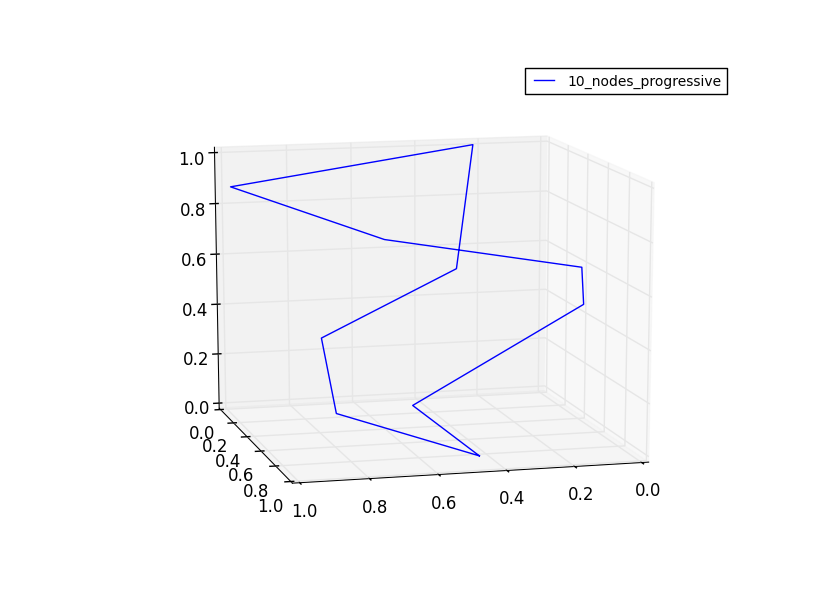
\includegraphics[width=0.44\textwidth]{figures/10_nodes_progressive.png} 
		\label{fig:10_nodes_progressive}
	}
	\subfigure[20 Nodes Progressive]{
		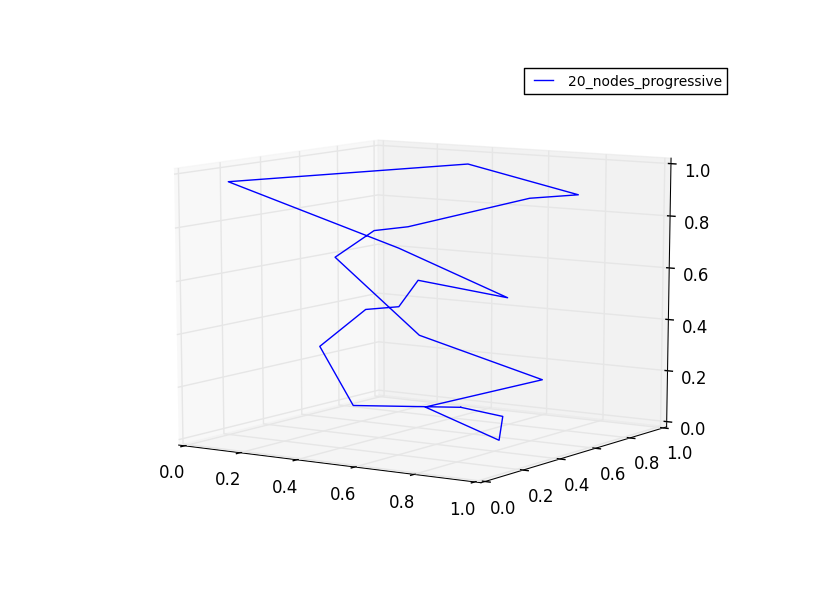
\includegraphics[width=0.44\textwidth]{figures/20_nodes_progressive.png} 
		\label{fig:20_nodes_progressive}
	}
	\subfigure[60 Nodes Progressive]{
		\includegraphics[width=0.44\textwidth]{figures/60_nodes_progressive.png} 
		\label{fig:60_nodes_progressive}
	}
	\subfigure[100 Nodes Progressive]{
		\includegraphics[width=0.44\textwidth]{figures/100_nodes_progressive.png} 
		\label{fig:100_nodes_progressive}
	}
	\caption{Exact routes calculated by travelling salesman}
	\label{fig:exact_routes_calculated_by_travelling_salesman}
\end{figure}

Figure \ref{fig:exact_routes_calculated_by_travelling_salesman} shows a number of optimal routes for varying numbers of nodes whose order is defined by the progressive travelling salesman algorithm. For the 100 node route it is difficult to see the exact routing; however for the other routes a logical approach to the routing problem can be seen. The initial progressive travelling plane logic did not produce routes of this quality as the least cost route on the way up would always favour finishing lower down even though in the next iteration this would mean having to gain greater height. Due to this visual identification of problems the cost of travel to the highest node is added to the up path for each iteration. This improvement caused the results that are shown.

Figure \ref{fig:20_nodes_progressive} displays some imperfections in the calculation of an optimal route. This is due to the significant change in height experienced at the top section of the route (where the routes A and B join up to form a single route). This suggests that figures \ref{fig:60_nodes_progressive} and \ref{fig:100_nodes_progressive} could contain inefficiencies in the route.

\subsection{Path Planning}
\label{sec:path_planning}

The least energy route through a number of nodes has been defined; however this route assumes that the UAV is able to turn on the spot and is not constricted by turning radius. Therefore to compute the actual energy cost of circumnavigating a route the turning radius of the UAV needs to be considered. Dubins paths can be used to produce a path from this route.

To compute a path through a sample volume the altitude of the unmanned aerial vehicle must be taken into consideration. The assumption for this stage in path planning is that the plane considered is able to change its rate of climb quick enough to approximate being instantaneous, whereas the rate of turn is not able to change with the same speed.

To increase the accuracy of this assumption the rate of climb for each section would change gradually from the previous section's rate of climb to the next section's rate of climb. However given the added complexity of this implementation it was assumed that the improvement on accuracy would not be sufficient to warrant the time required.

\begin{figure}
	\centering
	
	\subfigure[10 Node Path]{
		\includegraphics[width=0.44\textwidth]{figures/10_node_path.png} 
		\label{fig:10_node_path}
	}
	\subfigure[20 Node Path]{
		\includegraphics[width=0.44\textwidth]{figures/20_node_path.png} 
		\label{fig:20_node_path}
	}
	\caption{UAV Routes and Paths through Latin Hypercubes}
	\label{fig:uav_routes_and_paths_through_latin_hypercubes}
\end{figure}

Figure \ref{fig:10_node_path} shows the optimal path and route for a UAV to circumnavigate a 10 node Latin hypercube. The route is calculated before the path and then the path is calculated from the heading at each node in the route. From visual observation of the route it looks to be an optimal ordering of nodes and the path selected through the nodes adheres to the flight characteristics of a plane.

Figure \ref{fig:20_node_path} shows the optimal path and route for a UAV to circumnavigate a 10 node Latin hypercube calculated in the same manner as the previous. Though this path is harder to visually inspect it looks to follow a path with limited change in height. In addition for each change in direction the flight characteristics are taken into account.

\section{Results}
\label{sec:results}

\subsection{Energy Model Results}
\label{sec:energy_model_results}

In section \ref{sec:energy_model} an energy model for the flight of a plane was defined. The varying coefficients of lift and drag were investigated to validate the iterative approach to define the Reynolds number. An example plane was selected to test whether the results for this model are viable. The energy coefficients of the plane considered defines the values taken forward in the report.

\begin{table}[width=\textwidth]
\centering

    \begin{tabular}{ll}
    Air Foil Name	& naca23015-il	\\
Mass $(kg)$	& $m = 0.64$	\\
Oswald Factor	& $e = 0.7$	\\
Wing Area $(m^2)$	& $S = 0.204$	\\
Wing Span $(m)$	& $b = 1.50$	\\

    \end{tabular}
\caption{Table of Plane Properties}
\label{tbl:table_of_plane_properties}
\end{table}

Table \ref{tbl:table_of_plane_properties} shows the properties of the plane considered. Aside from the name of the airfoil and the Oswald factor, all the parameters are readily available specifications that can be found on many out of the box UAVs. The airfoil was to be specified in order to obtain an estimation for the coefficients of lift and drag. The Oswald factor displayed in this table is also an estimation for the given plane; however for the purpose of this analysis is probably sufficient.

\begin{table}[width=\textwidth]
\centering

    \begin{tabular}{ll}
    Aspect Ratio	& $11.03$	\\
Wing Chord $(m)$	& $0.14$	\\

    \end{tabular}
\caption{Table of Calulated Plane Properties}
\label{tbl:table_of_calulated_plane_properties}
\end{table}

Table \ref{tbl:table_of_calulated_plane_properties} shows a number of calculated properties from the initial data. The aspect ratio was calculated using  $A = \frac{b^2}{S}$ and the wing chord was calculated using $c = \frac{S}{b}$. This allowes for any plane whose data can be fitted to the data in table \ref{tbl:table_of_plane_properties} to be used for this energy model.

Given the main driving variable of analysis is the energy coefficient $\beta$, the energy coefficient output from the energy model was investigated. The flight velocity defines how great the drag force is that the plane works against in normal flight; therefore this was used as the driving variable to analyse the changing energy coefficient.

\begin{figure}
\centering
\includegraphics[width=0.6\textwidth]{figures/flight_velocity__v__and_energy_coeficient__beta_.png} 
\caption{Flight Velocity $V$ and Energy Coeficient $\beta$}
\label{fig:flight_velocity_v_and_energy_coeficient_beta_}
\end{figure}

Figure \ref{fig:flight_velocity_v_and_energy_coeficient_beta_} shows the variation of the energy coefficient with flight velocity. The separate series define when the Reynolds number used to obtain the foil data has changed due to the velocity change. The Reynolds number can be plotted as a separate series as it is returned when the velocity of the plane is altered. For actual flight this curve would be a single line; however as the data sets are only available for certain Reynolds numbers the inconsistencies are present.

The velocity that yields the greatest range given the plane considered is $V = 10.7 ms^{-1}$ at this flight velocity the energy coefficient takes the value $\beta = 0.10$. For investigation of climbing and turning flight this is the flight velocity considered.

\begin{figure}
\centering
\includegraphics[width=0.6\textwidth]{figures/energy_cost_of__180circ__turn_at__107_ms1_.png} 
\caption{Energy Cost of $180^{\circ}$ Turn at $10.7 ms^{-1}$}
\label{fig:energy_cost_of_180circ_turn_at_107_ms1_}
\end{figure}

Figure \ref{fig:energy_cost_of_180circ_turn_at_107_ms1_} shows the variation in the cost of the plane detailed in table \ref{tbl:table_of_plane_properties} navigating a $180^{\circ}$ turn with varying turning radiuses. The varied turning radiuses cause the distance travelled to vary hugely. Thus if this analysis was only done with the circular distance of the turn, the cost would mainly be affected by this distance travelled. Therefore for this analysis the plane is assumed to start at one point, then, travel in a straight line until initiating a turn which passes through a second point half way round the turn before finishing the turn and flying back to be level with the initial point. This means as the turning radius is increased the straight line flight is decreased.

It can be seen from figure \ref{fig:energy_cost_of_180circ_turn_at_107_ms1_} that the energy consumed in turning $180^{\circ}$ reduces to an optimal at a given turning radius. This is due to the lesser forces required on the plane to turn with a greater turning circle. This finding needs to be considered when it comes to path planning.

\begin{figure}
\centering
\includegraphics[width=0.6\textwidth]{figures/energy_cost_of_flight_with_horizontal_distance__10m__and_varyed_vertical_distance_at__107_ms1_.png} 
\caption{Energy Cost of Flight with Horizontal Distance $10m$ and Varyed Vertical Distance at $10.7 ms^{-1}$}
\label{fig:energy_cost_of_flight_with_horizontal_distance_10m_and_varyed_vertical_distance_at_107_ms1_}
\end{figure}

Figure \ref{fig:energy_cost_of_flight_with_horizontal_distance_10m_and_varyed_vertical_distance_at_107_ms1_} shows the variation of the cost for the plane detailed in table \ref{tbl:table_of_plane_properties} to climb for a horizontal distance of $10m$ over varied climb heights. Here the horizontal distance is maintained at a constant and the vertical distance is increased to determine the extra flight cost. It can be seen that cost varies fairly linearly with climb height. This relationship is not truly accurate as it does not account for the reduction in aerodynamic efficiency which results from a greater angle of attack that is required for a greater climb angle. 

The results to the energy model are as expected given the simplicity of the model utilised; however there is room for improvement on the accuracy of how the model predicts climbing and turning flight consumption. The framework for allowing any angle of attack to be pulled from the internet makes this improvement easy to facilitate.

\subsection{Progressive Travelling Plane}
\label{sec:progressive_travelling_plane_0}

In section \ref{sec:progressive_travelling_plane} a best guess approach to the TSP was presented with specific application to the flight of a plane. This provided a method to calculate the order in which nodes should be visited for the lease cost route. The method was sufficiently computationally simple so that routes could be found through large numbers of nodes.

To test the progressive algorithm fully the input parameters that affect its operation were varied to consider how they affected the resulting best guess cost. The following parameters affect the operation of the progressive travelling plane algorithm:

\begin{itemize}
\setlength{\itemsep}{-12pt}
\item Number of nodes sample plan $N$
\item Number of nodes in subset $n$
\item Energy coefficient $\beta$

\end{itemize}

Before considering the quality of the model produced the parameters affecting the computation time were investigated. This allowed the further investigation of parameters to stay within reasonable limits. The energy coefficient does not change the computation time as the problem is the same complexity but it drastically changes the optimal ordering.

\begin{table}[width=\textwidth]
\centering

    \begin{tabular}{lllll}
    Nodes in sample $N$	& 10	& 10	& 10	& 10	\\
Nodes in subset $n$	& 2	& 3	& 4	& 5	\\
Computation time $(ms)$	& 2	& 3	& 52	& 4083	\\
Best route cost $(m)$	& 1.27	& 1.26	& 1.22	& 1.22	\\

    \end{tabular}
\caption{Comparison of route calculation}
\label{tbl:comparison_of_route_calculation_0}
\end{table}

Table \ref{tbl:comparison_of_route_calculation_0} shows the effect of increasing the number of nodes considered in the subset, where subset refers to the number of nodes that are considered in each route of the progressive iteration of two routes. It is apparent that the computation time increases dramatically as seen in the exact TSP as the number of nodes in the subset is increased. This means computationally this method is not viable beyond 4 nodes in each route in the subset.

\begin{table}[width=\textwidth]
\centering

    \begin{tabular}{lllll}
    Nodes in sample $N$	& 10	& 20	& 60	& 100	\\
Nodes in subset $n$	& 4	& 4	& 4	& 4	\\
Computation time $(ms)$	& 52	& 179	& 725	& 1315	\\
Best route cost $(m)$	& 1.22	& 1.4	& 2.47	& 3.61	\\

    \end{tabular}
\caption{Comparison of route calculation}
\label{tbl:comparison_of_route_calculation_1}
\end{table}

Table \ref{tbl:comparison_of_route_calculation_1} shows the effect of increasing the total number of nodes in the routing problem while maintaining the number of nodes in the subset at a constant. It can be seen that for 100 nodes in the subset the computation time remains manageable as it did not increase drastically with greater numbers of nodes in the total sample.

The computation requirement of the progressive TSP is more than acceptable. However the routes produced may not be sufficiently close the actual optimum. Visual inspection of the given routes suggested that the logic is sound however the cost needs to be compared with the cost of the absolute optimal route. This is done by computing the costs of all routes using the exact TSP and then comparing.

\begin{figure}
\centering
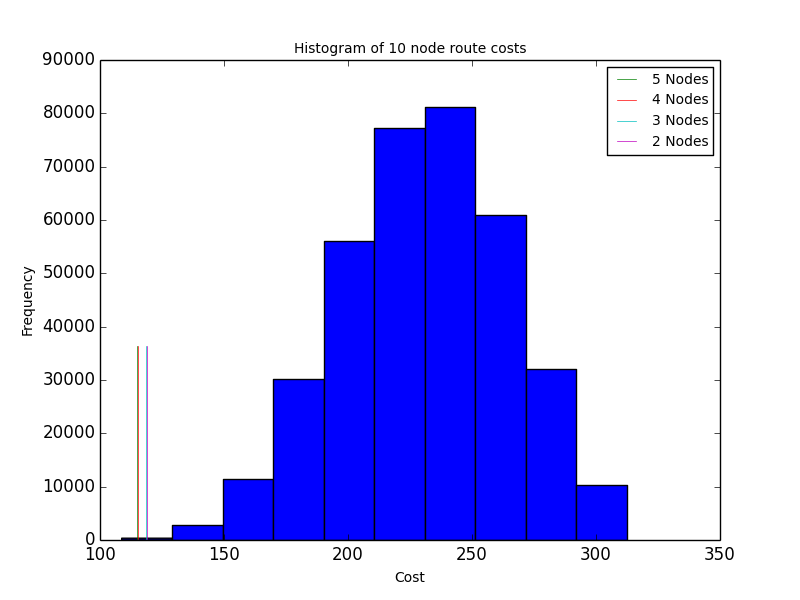
\includegraphics[width=0.6\textwidth]{figures/histogram_of_10_node_route_costs.png} 
\caption{Histogram of 10 node route costs}
\label{fig:histogram_of_10_node_route_costs}
\end{figure}

Figure \ref{fig:histogram_of_10_node_route_costs} shows a histogram of different route costs for a 10 node Latin hypercube. The lines on this histogram plot represent the best cost routes with different numbers of nodes in the subset. It can be seen that the cost of the best route from the progressive approach closely approaches the optimal solution as calculated using the exact TSP.

The minimum cost route for the exact travelling plane was $1.14m$ while the minimum cost for the progressive travelling plane was $1.22m$; a figure is within $7\%$. In terms of ranking the best guess result ranks 28 out of 362880 results. Which means the progressive best cost route is within $0.01\%$ of the rankings of all possible routes. Therefore for a 10 node route with the energy coefficient $\beta=0.1$ the progressive travelling plane approach is very much acceptable.

To fully test validity the progressive travelling plane route planner should have been compared with the exact results for Latin hypercubes with a number of nodes greater than 10; however the computation costs of a more than 10 node routes makes this not a viable option. As an alternative, the relative cost decrease of adding more nodes can be considered.

\begin{figure}
\centering
\includegraphics[width=0.6\textwidth]{figures/comparison_of_relative_route_costs_for_progressive_travelling_plane.png} 
\caption{Comparison of Relative Route Costs for Progressive Travelling Plane}
\label{fig:comparison_of_relative_route_costs_for_progressive_travelling_plane}
\end{figure}

Figure \ref{fig:comparison_of_relative_route_costs_for_progressive_travelling_plane} shows how the relative route cost varies with the number of nodes in the subset. Relative route cost refers to the cost as a percentage of the minimum cost achieved. It has to be noted at this point that the minimum cost achieved is not the actual minimum cost route. However it does mean the relation of the other costs can be seen to the best computable cost and allows for comparison between vastly different numbers of nodes. From looking at this figure it can be seen that routes with less total nodes generally plateau within the range of the subset numbers investigated. This shows that the result achieved approaches some form of minimum. However, given the computational time to compute a route with 6 node subsets is vast this is the furthest this analysis can be taken.

For the investigated energy coeficient $\beta = 0.1$ at low nodes the progressive TSP yields good results. However, given the energy coefficient $\beta$ depicts the relative cost of level vs inclined flight and that the progressive travelling planes is based on route planning through height order; changing this coefficient could have a big effect on the quality of the progressive approach.

\begin{figure}
\centering
\includegraphics[width=0.6\textwidth]{figures/best_costs_of_routes_through_10_node_latin_hypercubes_with_varying_energy_coeficients.png} 
\caption{Best Costs of Routes through 10 Node Latin Hypercubes with Varying Energy Coeficients}
\label{fig:best_costs_of_routes_through_10_node_latin_hypercubes_with_varying_energy_coeficients}
\end{figure}

Figure \ref{fig:best_costs_of_routes_through_10_node_latin_hypercubes_with_varying_energy_coeficients} shows how the progressive and exact travelling plane results are affected by changing the energy coefficient $\beta$. From looking at the results in this figure it can be seen that the progressive travelling plane approach holds true even when the energy coefficient is varied.

The progressive travelling plane approach to route planning has been validated under varying parameters with links to the exact travelling plane model. An attempt has been made to verify that the quality of the results hold true for larger numbers of nodes however due to the inability to test this hypothesis directly this is not verified. The computational efficiency of the progressive TSP has been found to be far better than that of the exact TSP. As a result of these factors and given the extent of this analysis, the progressive TSP is acceptable to take forward to the next stage of the project.

\subsection{Path Planning}
\label{sec:path_planning_0}

In section \ref{sec:path_planning} Dubins paths were utilised to produce navigable routes from a set of ordered nodes. The paths produced passed visual inspection of validity. The resulting effect on both path length and energy consumption are investigated to consider the importance of path planning for UAVs.

\begin{figure}
\centering
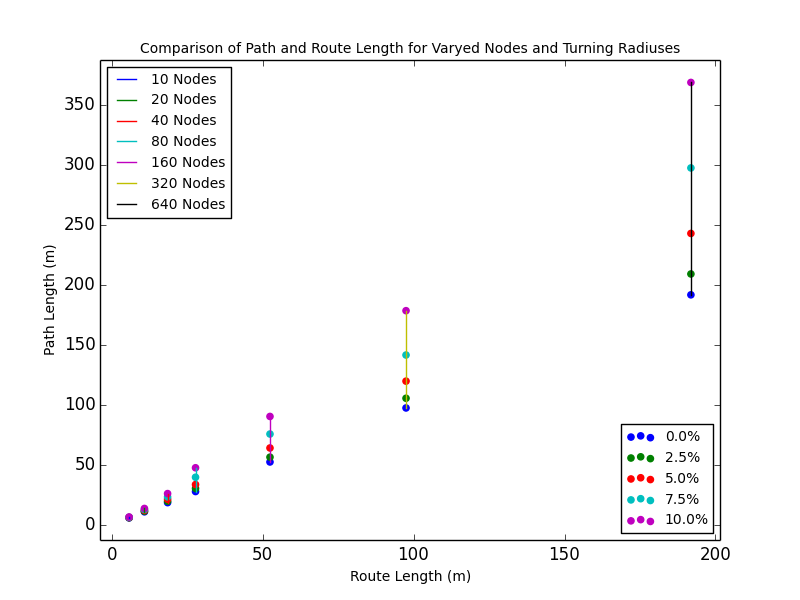
\includegraphics[width=0.6\textwidth]{figures/comparison_of_path_and_route_length_for_varyed_nodes_and_turning_radiuses.png} 
\caption{Comparison of Path and Route Length for Varyed Nodes and Turning Radiuses}
\label{fig:comparison_of_path_and_route_length_for_varyed_nodes_and_turning_radiuses}
\end{figure}

Figure \ref{fig:comparison_of_path_and_route_length_for_varyed_nodes_and_turning_radiuses} shows the relationship between the route length and path length for a number of different Latin hypercubes. For each Latin hypercube the distance of the shortest route (length of ordered route through nodes) and a number of shortest paths (length of path through ordered nodes that takes into account the flight characteristics of the plane) have been calculated and compared. The shortest paths are considered with turning radiuses varied between $0\%$ and $10\%$ of the length of the side of the area that is being explored. For this analysis the area of interest is a unit cube and the percentage value represents the maximum turning radius of the plane over the length of one axis.

It can be seen from figure \ref{fig:comparison_of_path_and_route_length_for_varyed_nodes_and_turning_radiuses} that as the number of nodes in the Latin hypercube is increased (vertical coloured lines indicate a set of tests on a single Latin hypercube) the effect of increased turning radius (turning radius is indicated by sets of coloured points) also increases. For the case where the turning radius is $0\%$ the path length and route length are the same as the UAV can affectively turn on the spot. Given the size of the research area that will be utilised for collecting atmospheric data using a UAV the added distance due to path length will have a negligible effect on the final distance. The stage at which this consideration may be required to be considered is in computing the final energy of the path. This is due to the greater accuracy of energy cost being required at this stage.

To utilise the path planning component in computing a best estimation of the energy consumed along the path, the energy as a result of turning radius needs to be considered along with that of level and turning flight. The energy consumed in a turn is a result of the severity of the turn and the distance travelled in that turn. The energy model presented in section \ref{sec:energy_model} was able to compute the energy cost of navigating a turn at a given radius. The energy consumed was found to have an optimal value where the balance between high force turning angle and long distance turning against drag were at a minimum. For the path planning problem the effect of the turning radius must be considered.

\begin{figure}
\centering
\includegraphics[width=0.6\textwidth]{figures/total_path_energy_for_route_through_20_node_latin_hypercube_with_changing_turning_radius.png} 
\caption{Total Path Energy for Route through 20 Node Latin Hypercube with Changing Turning Radius}
\label{fig:total_path_energy_for_route_through_20_node_latin_hypercube_with_changing_turning_radius}
\end{figure}

Figure \ref{fig:total_path_energy_for_route_through_20_node_latin_hypercube_with_changing_turning_radius} shows the variation of path energy through a 20 node Latin hypercube at 10m/s as a result of altered turning radius. It can be seen that the turning radius affects the total energy consumed on the route and has an optimal value. This optimal value is a product of the spacing of the nodes in the sample plan and the velocity of the plane. The variation in energy as a percentage of the minimum energy experienced is only 0.53\% therefore the variation of turning radius on the energy cost is sufficiently negligible to disregard.

\begin{figure}
\centering
\includegraphics[width=0.6\textwidth]{figures/percentage_path_energy_for_routes_through_a_number_of_node_latin_hypercubes_with_changing_turning_radius.png} 
\caption{Percentage Path Energy for Routes through a Number of Node Latin Hypercubes with Changing Turning Radius}
\label{fig:percentage_path_energy_for_routes_through_a_number_of_node_latin_hypercubes_with_changing_turning_radius}
\end{figure}

Figure \ref{fig:percentage_path_energy_for_routes_through_a_number_of_node_latin_hypercubes_with_changing_turning_radius} shows the variation of the path energy as a result of varied turning radiuses and number of nodes in the sample plan. This figure is to illustrate the effect of node spacing on the energy consumption of a path. The Latin hypercubes with greater numbers of nodes have closer packed nodes therefore the lower turning radiuses are more optimal. The percentage change to the energy of the route is negligible as a result of increase turning radius however this is purely illustrative of the effect of node spacing. The energy percentage here is the energy as a percentage value of the energy required for a route with a turning radius of unity.

\begin{figure}
\centering
\includegraphics[width=0.6\textwidth]{figures/percentage_path_energy_for_route_through_22_node_latin_hypercube_with_changing_turning_radius_and_flight_velocity.png} 
\caption{Percentage Path Energy for Route through 22 Node Latin Hypercube with Changing Turning Radius and Flight Velocity}
\label{fig:percentage_path_energy_for_route_through_22_node_latin_hypercube_with_changing_turning_radius_and_flight_velocity}
\end{figure}

Figure \ref{fig:percentage_path_energy_for_route_through_22_node_latin_hypercube_with_changing_turning_radius_and_flight_velocity} shows the variation of total path energy as a result of varied turning radiuses and flight velocities. This figure is to illustrate the effect of flight velocity on the energy consumption of a path. The energy percentage here is the energy as a percentage value of the energy required for a route with a turning radius of unity. It can be seen that the greater the flight velocity the higher the optimal turning radius is. This figure displays percentage values as the energy increases drastically given greater flight velocities.

The path planing component of this report allows the energy consumed by a UAV in navigating a sample plan to be more accurately calculated as the effect of the turning radius can be investigated. This means the path to be optimised for the best turning radius given a route. Additionally the findings outline the potential for the turning radius to be optimised for least energy consumed based on a node by node basis, this suggestion is due to the optimal turning radius being dependent on node spacing therefore should be calculated per node as the distance between each node is very different. For the continuation of this project the added energy consumption due to the UAV flight path will be disregarded as the energy consumption is not vastly different to that of the route for large turning radiuses in comparison to the research area.

\subsection{Sample Plan Model}
\label{sec:sample_plan_model}

Thus far in the report routes have been found from a collection of nodes in particular sampling plans, the number of nodes in the sampling plan along with the area of interest affects the length of the route through the points and the total height change experienced. These two factors then go to calculating the total energy expenditure of the route. The desired design route is to calculate the desired route given the area of interest and total energy of the plane. This requires the relationship between the length, width and height of the research area and the number of nodes in the sample plan to the resulting energy cost of the route to be modelled.

The problem with computing this relationship is that the route through the sample area is dependent upon the energy model for a given plane. As in the extremes the energy model can completely favour either climbing flight or level flight.

To compute a model for each Latin hypercube a sampling plan was defined with 100 test cases this sampling plan ranged between 0 and 1000 in each vertex. These sampling plans provide for the most efficient way to collect data on each Latin hypercube. For each Latin hypercube with between 20 and 120 nodes all test cases are analysed to return the exact energy cost. This energy cost can then be related to the research volume for each set of node numbers.

\begin{figure}
\centering
\includegraphics[width=1\textwidth]{figures/data_model_diagram.png} 
\caption{Diagram of Sample Plan Model Logic}
\label{fig:data_model_diagram}
\end{figure}

Figure \ref{fig:data_model_diagram} shows the logic required to plan a route based on the total energy available. In this diagram the calculation of model variables is shown in the process. However if these variables were required to be calculated on the fly this would not be a viable approach. In addition if this were to be calculated each and every time the exact research area would be used for each number of nodes, as opposed to 100 samples which are used to return a model for the varying route cost given a number of nodes.

\begin{figure}
\centering
\includegraphics[width=0.6\textwidth]{figures/scatter_plot_of_varying_route_and_path_lengths_for_a_100_node_latin_hypercube_model.png} 
\caption{Scatter plot of varying route and path lengths for a 100 node Latin hypercube model}
\label{fig:scatter_plot_of_varying_route_and_path_lengths_for_a_100_node_latin_hypercube_model}
\end{figure}

Figure \ref{fig:scatter_plot_of_varying_route_and_path_lengths_for_a_100_node_latin_hypercube_model} shows the relationship between the research area ($x 	imes y$), research height ($z$) and the resulting route cost. This depicts that the energy required to circumnavigate a 100 node Latin hypercube, varies non linearly with both the area and height. This figure shows that the model needs to be computed from both the length and width as opposed to the area however this form allows for depiction on a figure.

\begin{equation}
\label{eq:energy_equation_0}
E=MA\cdot (xy)^{EA}+MD\cdot abs(x-y)+MZ\cdot z^{EZ}+C
\end{equation}

Equation \ref{eq:energy_equation_0} shows the format of how the length, width and height of the research area affect the route cost. For every number of node, Latin hypercube and energy coefficients different model parameters are required to correctly depict the relation between the dimension inputs and the energy cost.

\begin{equation}
\label{eq:100_node_energy_equation}
E=0.15(xy)^{0.708}+0.75abs(x-y)+0.50z^{1.064}+282
\end{equation}

Equation \ref{eq:100_node_energy_equation} shows how the length, width and height of the research area affects the route energy for a route determined by the energy coefficient 0.1 through a 100 node Latin hypercube. The parameters here are calculated using a least squares regression function.

To calcualte the actual route energy from this cost the energy factor gamma is required. The route cost can simply be multiplied by gamma for the plane considered for routing and this model produces the total route cost for a particular plane without having to compute all costs of routing round different Latin hypercubes.

\begin{figure}
\centering
\includegraphics[width=0.9\textwidth]{figures/energy_model_prediction_compared_with_calculated_energies_for_energy_coeficient__beta__01_.png} 
\caption{Energy Model Prediction Compared with Calculated Energies For Energy Coeficient $\beta = 0.1$}
\label{fig:energy_model_prediction_compared_with_calculated_energies_for_energy_coeficient_beta_01_}
\end{figure}

Figure \ref{fig:energy_model_prediction_compared_with_calculated_energies_for_energy_coeficient_beta_01_} shows the comparison of the desired route energy and the resulting route energy for the energy coefficient $\beta = 0.1$. The inclined line through the data shows the optimal result where the prediction is completely accurate. This data is obtained from randomly varying the research area and the desired energy consumption and then computing the number of nodes that are predicted to make up the route that is optimal. The actual energy of this route is then calculated exactly and plotted in comparison to the desired route. The series represent the number of nodes used to produce the routes.

The predictions seen for the case where $\beta=0.1$ are on average out by 4.72\% of the desired route energy. This suggests that for this energy coefficient the model produced is viable to accurately select a sampling plan given a required energy consumption. This may not be the case for other energy coefficients due to the drastic affect the energy coefficient has on the routing problem.

\begin{figure}
	\centering
	
	\subfigure[$\beta = 0.2$]{
		\includegraphics[width=0.3\textwidth]{figures/_beta__02_.png} 
		\label{fig:beta_02}
	}
	\subfigure[$\beta = 0.3$]{
		\includegraphics[width=0.3\textwidth]{figures/_beta__03_.png} 
		\label{fig:beta_03}
	}
	\subfigure[$\beta = 0.4$]{
		\includegraphics[width=0.3\textwidth]{figures/_beta__04_.png} 
		\label{fig:beta_04}
	}
	\caption{Energy Model Prediction Compared with Calculated Energies For Varying Energy Coeficients $\beta$}
	\label{fig:energy_model_prediction_compared_with_calculated_energies_for_varying_energy_coeficients_beta}
\end{figure}

Figure \ref{fig:energy_model_prediction_compared_with_calculated_energies_for_varying_energy_coeficients_beta} shows the comparison of desired and actual route energies for random sample areas and desired route energies for the energy coefficients $\beta =$ 0.2, 0.3 and 0.4. It can be seen that as the energy coefficient is increased the prediction accuracy for the route becomes less viable. Given these predictions are for specific values of the energy coefficient these results would get less accurate given any value for the energy coefficient being utilised. This would be the case for real implementation as the value for the energy coefficient is precisely defined from the plane energy model.

\begin{table}[width=\textwidth]
\centering

    \begin{tabular}{llll}
    Figure	& Energy Coeficient $(\beta)$	& Prediction Error	& Prediction Standard Deviation	\\
\ref{fig:energy_model_prediction_compared_with_calculated_energies_for_energy_coeficient_beta_01_}	& $0.1$	& 4.72\%	& 3.90\%	\\
\ref{fig:beta_02}	& $0.2$	& 7.95\%	& 6.98\%	\\
\ref{fig:beta_03}	& $0.3$	& 11.87\%	& 11.86\%	\\
\ref{fig:beta_04}	& $0.4$	& 12.62\%	& 11.53\%	\\

    \end{tabular}
\caption{Table of Results}
\label{tbl:table_of_results}
\end{table}

Table \ref{tbl:table_of_results} shows the prediction error variation as a result of varying the value of the energy coefficient. It can be seen that the model predictions are only viable for low values of the energy coefficient. Therefore the model is of an acceptable accuracy to be utilised in the model predictions for low values of the energy coefficient. Given the UAV considered in this report has a low energy coefficient at optimal range velocity this suggests that this model would be acceptable for use within path planning for the purpose of collecting atmospheric data using UAVs, as this enables a research area to be specified and a suitable Latin hypercube to be selected given the desired total energy expenditure.

\section{Conclusions}
\label{sec:conclusions}

This report has looked at collection of atmospheric data using UAVs with specific focus on collecting the best set of sample data for a given research area while maximising utlisation of the energy contained within the plane. To complete this task Latin hypercubes were used to provide optimal space filling sampling plans and then the least cost route, with the path then calculated through the Latin hypercubes. To enable planning from the basis of the required energy consumption, the plane's energy consumption was modelled in a mannar where a single coefficient defines the route characteristics. This enabled a model to be produced from multiple tests that can predict the energy consumed based on the number of nodes in the Latin hypercube. This provides for the best spread of data collection and adheres to the UAV energy requirement.

\subsection{Energy Model}
\label{sec:energy_model_0}

The energy model produced uses the most simplified aerodynamic equations to determine the cost of navigating a certain path. Given the simplicity of the energy model, routing can be characterised based on a single variable which can be used in a sample model that determines the optimal number of nodes. The coefficients of lift and drag selected for the plane do not accurately portray the real values that will be experienced as they are pulled for purely the airfoil in question. For the routing component of this project the ranking of energy cost is taken to be more important than actual cost this is acceptable. However the drag effects of the plane fuselage need to be accounted for otherwise a route calculated would far exceed the predicted energy. The values utilised for the air density and viscosity in this model assume that they remain constant at all altitudes in the research area which is not an accurate assumption when altitude varied greatly.

\subsection{Travelling Plane}
\label{sec:travelling_plane}

The progressive approach to the TSP yields a good estimation as to the least cost path to navigate a number of nodes. This enables route planning with numbers of nodes that would not be possible using the exact travelling salesman. Therefore the calculation produced is of significant value. The limitation lies in how many nodes the planning can be relied upon to route though while maintaining a best guess cost. Due to the inability to collect data on the perfect solution for more than 10 nodes I have found no sound method for substantiating routing though a 100 node hypercube. The quality of results obtained in the tests performed suggested this route logic to be solid for what has been tested though. This approach provides what it set out to accomplish which is a best guess solution to route planning that is sufficient to be confident of this routing algorithm for the basis of the subsequent calculations

\subsection{Path Planning}
\label{sec:path_planning_1}

Utilising Dubins paths to take into account the flight characteristics of the plane enables the energy model to be applied more accurately and the turning radius to be optimised according to the increased consumption related to the bank angle of the turn. Dubins paths are well documented solutions to the problem of vehicle paths and there has been previous literature on applying them in three dimensions. Therefore the shortest distance paths calculated in this report are likely to be correct as any issues can be visually defined. However in light of analysis the shortest Dubins paths do not always correspond to the least energy path due to the increased energy required for a smaller turning radius. Working to improve the implementation of these paths is important as this project strives to compute an as accurate as possible energy cost.

\subsection{Data Model}
\label{sec:data_model}

The data model calculated works well for low values of the energy consumption coefficient that directly correspond to the energy coefficient used to produce the model. However for higher values of the coefficient or in-between two tests where there is a lack of data from previous tests the model is not accurate enough for utilisation. With enough test cases where the energy coefficient is varied using a four dimension sampling plan not just the three dimensions which define the area of interest, the model produced is likely to hold sufficient worth to confidently predict costs for any low energy coefficient, not just coefficients that lie in previously tested conditions. The correlations of the sample model are only viable in the confines of the current energy model therefore an improvement on the energy model would require updating the sample model to reflect the added complexity.

\subsection{Looking Forward}
\label{sec:looking_forward}

The approaches documented here are far from a perfect approach to the problem of collecting atmospheric data. However the combination of sampling plans and the progressive travelling plane approach to path planning for atmospheric data collection presents an interesting foothold for further investigation. In addition the proof that, in its simplest form a model can be produced that allows planning from the basis of the required energy consumption, facilitates the potential (however small) for this work to be utilised in actual path planning for atmospheric data collection.

An initial aim of the project was to include consideration for uniform wind which would make the path planning presented here closer to the optimal. Dubins paths in the wind frame of reference correspond to trichordial path segments in the ground frame of reference. This would require a further geometrical calculation to enable this consideration to the path planing. In terms of the routing problem a previous energy model for this project included the consideration on computing the line integral through a vector field that allowed the distance of travel to be altered for the prevailing wind. This means that the cost of travel from nodes could be altered to consider even a non-uniform wind, however was not included for the final report due to the complexities of implementation.

Given the energy model is the basis for all routing consideration in this project, a non-linear approach to energy modelling would have the facility to correctly ascertain the cost of not just changing height but consider the rate at which the rate of height change can occur. But such non-linear version of the energy model would not be viable in the route planning stage as the cost of travel between nodes is considered as individual components. However upon calculation of the path, a non-linear energy model could provide a far more accurate method to defining the exact energy required by a UAV.

\section{Report Methodology}
\label{sec:report_methodology}

\subsection{Project Management and Organisation}
\label{sec:project_management_and_organisation}

To complete the objectives of this project while allowing sufficient time for each step careful project management was required. To produce a project plan the objectives of the project were considered and broken down into the elements that were required to complete each stage. The prerequisite requirements of each item in the project plan were then defined to ensure that each step could be completed when required. These requirements led to a framework for a project plan that only required estimation of the time required for each stage to be complete.

\begin{figure}[H]
\centering
\includegraphics[width=0.8\textwidth]{figures/project_plan.png} 
\caption{Gantt Chart of Project Plan}
\label{fig:project_plan}
\end{figure}

Figure \ref{fig:project_plan} shows the project plan followed.  The steps are on the left and the time which is allocated for completion indicated by coloured squares. This plan was not followed to the letter as some of the stages were more complicated than first imagined so a more gradual approach to developing the solution was required. These overruns were either due to more detailed literature analysis being required or continued trial and error on the part of programming the solution.

\subsection{Writing the Report}
\label{sec:writing_the_report}

The consideration and thought that went into composing ideas in the report often led to further analysis on the part of the code produced, it therefore seemed logical to produce the report in a more adaptive manor. This resulted in designing a parametric report where calculations, results and figures were automatically updated upon each run.

The adaptive report is written in python as all other project elements were computed using python. The basis of the logic is a TexDocument class that has a number of methods that deal with adding basic elements to a LaTeX document. Within the main content document these methods can easily be called to define: sections, paragraphs, figures, equations and tables. All these elements are added to a working LaTeX document as they are interpreted. Upon completion of the report the compile method can be called which calls pdfTex and BibLaTeX to build the pdf and automatically open it to view. In addition to standard features this approach means that: the LaTeX document automatically remunerates figure labels if there is repetition to ensure there is no cross over and nomeclature and abreviations can be collected within a dictionary from any point within the report.

Producing the report in this way means that whatever change of code was made can easily result in an updated report. The drawback however is the compute time required to compile the report. This problem was levitated using cached results to computations. The function loadOrRun within the shared module of the code for this project deals with caching of results. If parameters are changes then the cache automatically recalculates the required data. Additionally all display logic is run on each compile so a change in plot style is quick and easy to implement without having to recomputed the cache.

\section{Python Code}
\label{sec:python_code}

To use the functionality of this code the scipy stack is required. To enable writing of LaTeX files MikTex needs to be installed. If further Latin hypercubes need to be calculated MATLAB needs to run on the system. Calls to MikTex and MATLAB are wrtten on a windows computere so the cammand line calls are in windows syntax.

The python code included within the CD has the following modules:

\textbf{Shared} is a module that contains all the logic available that is required by all modules of the project and contains generic functions that could be used in all locations.

\textbf{Plane energy} is a module that is used to model the energy consumption of a plane. This module contains a number of global variables that define a default plane. A single class within this module is constructed using plane variables, this class is capable of computing the energy required for a number of flight manoeuvres and returning the energy coefficient and energy factor.

\textbf{Airfoil} is a module that is used to obtain data on a number of airfoils using \textit{airfoiltools.com}. The class contained within this module is constructed with a foil name and Reynolds number and can return the variation of the lift and drag coefficients with changing angle of attack.

\textbf{Latin hypercube} is a module that calls MATLAB to connect with the code produced by \citen{Forrester2008} and return Latin hypercube sampling plans of any given number of nodes and number of dimensions. The results to these MATLAB calls are cached to reduce the time of subsequent calls.

\textbf{Travelling plane} is a module that is used to calculate the least cost route through given nodes. The module contains both the exact all routes approach and the progressive travelling plane approach.

\textbf{Sample model} is a module that is used to compute models of the energy cost of a routes given different scenarios. This module enables the route planning for atmospheric data collection to be done from the requirement of total energy consumed.

\textbf{Dubins path} is a module used to compute the shortest distance Dubins paths either between two points with start and end directions defined or using the Dubins Path class the total path through a number of nodes. This module is not fully commented as the geometric logic is from \citen{Giese2012} and there is a lot of lines of code to explain.
\newpage
\bibliographystyle{unsrt}
\bibliography{references}
\newpage
\end{document}
